\begin{frame}{Exemplo de inserção utilizando \textit{hash} duplo}

    \begin{figure}
        \begin{tikzpicture}
            \draw (0, 1) grid (11, 2);

            \node at (0.5, 2.5) { \tt \footnotesize 0 };
            \node at (1.5, 2.5) { \tt \footnotesize 1 };
            \node at (2.5, 2.5) { \tt \footnotesize 2 };
            \node at (3.5, 2.5) { \tt \footnotesize 3 };
            \node at (4.5, 2.5) { \tt \footnotesize 4 };
            \node at (5.5, 2.5) { \tt \footnotesize 5 };
            \node at (6.5, 2.5) { \tt \footnotesize 6 };
            \node at (7.5, 2.5) { \tt \footnotesize 7 };
            \node at (8.5, 2.5) { \tt \footnotesize 8 };
            \node at (9.5, 2.5) { \tt \footnotesize 9 };
            \node at (10.5, 2.5) { \tt \footnotesize 10 };

            \node[anchor=west] at (1, 6) { \textit{Hash} duplo, $T = 11$ };
            \node[anchor=west] at (1, 5.5) { Elemento a ser inserido: \textcolor{blue}{$51$} };

        \end{tikzpicture}
    \end{figure}

\end{frame}

\begin{frame}{Exemplo de inserção utilizando \textit{hash} duplo} 

    \begin{figure}
        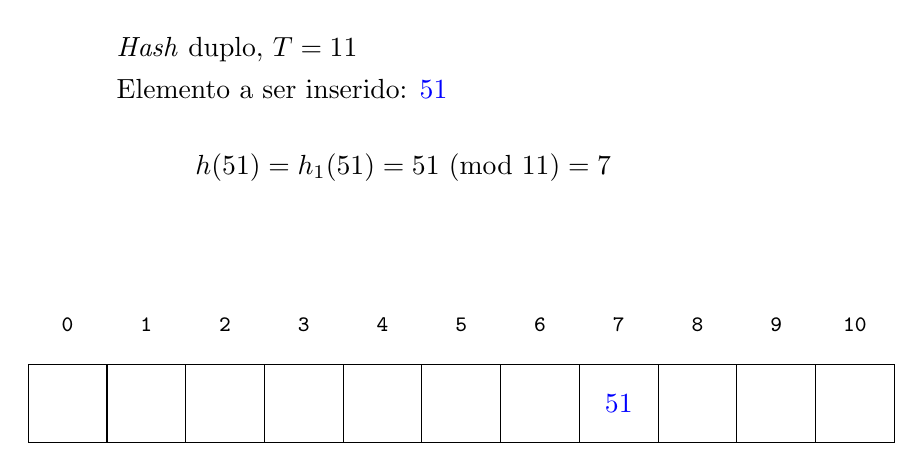
\begin{tikzpicture}
            \draw (0, 1) grid (11, 2);

            \node at (0.5, 2.5) { \tt \footnotesize 0 };
            \node at (1.5, 2.5) { \tt \footnotesize 1 };
            \node at (2.5, 2.5) { \tt \footnotesize 2 };
            \node at (3.5, 2.5) { \tt \footnotesize 3 };
            \node at (4.5, 2.5) { \tt \footnotesize 4 };
            \node at (5.5, 2.5) { \tt \footnotesize 5 };
            \node at (6.5, 2.5) { \tt \footnotesize 6 };
            \node at (7.5, 2.5) { \tt \footnotesize 7 };
            \node at (8.5, 2.5) { \tt \footnotesize 8 };
            \node at (9.5, 2.5) { \tt \footnotesize 9 };
            \node at (10.5, 2.5) { \tt \footnotesize 10 };

            \node[anchor=west] at (1, 6) { \textit{Hash} duplo, $T = 11$ };
            \node[anchor=west] at (1, 5.5) { Elemento a ser inserido: \textcolor{blue}{$51$} };

            \node[anchor=west] at (2, 4.5) { $h(51) = h_1(51) = 51\ (\mbox{mod}\ 11) = 7$ };

            \node at (7.5, 1.5) { \textcolor{blue}{$51$} };
        \end{tikzpicture}
    \end{figure}

\end{frame}

\begin{frame}{Exemplo de inserção utilizando \textit{hash} duplo} 

    \begin{figure}
        \begin{tikzpicture}
            \draw (0, 1) grid (11, 2);

            \node at (0.5, 2.5) { \tt \footnotesize 0 };
            \node at (1.5, 2.5) { \tt \footnotesize 1 };
            \node at (2.5, 2.5) { \tt \footnotesize 2 };
            \node at (3.5, 2.5) { \tt \footnotesize 3 };
            \node at (4.5, 2.5) { \tt \footnotesize 4 };
            \node at (5.5, 2.5) { \tt \footnotesize 5 };
            \node at (6.5, 2.5) { \tt \footnotesize 6 };
            \node at (7.5, 2.5) { \tt \footnotesize 7 };
            \node at (8.5, 2.5) { \tt \footnotesize 8 };
            \node at (9.5, 2.5) { \tt \footnotesize 9 };
            \node at (10.5, 2.5) { \tt \footnotesize 10 };

            \node[anchor=west] at (1, 6) { \textit{Hash} duplo, $T = 11$ };
            \node[anchor=west] at (1, 5.5) { Elemento a ser inserido: \textcolor{blue}{$16$} };

%            \node[anchor=west] at (2, 4.5) { $h(51) = 51\ (\mbox{mod}\ 11) = 7$ };

            \node at (7.5, 1.5) { \textcolor{black}{$51$} };
        \end{tikzpicture}
    \end{figure}

\end{frame}

\begin{frame}{Exemplo de inserção utilizando \textit{hash} duplo} 

    \begin{figure}
        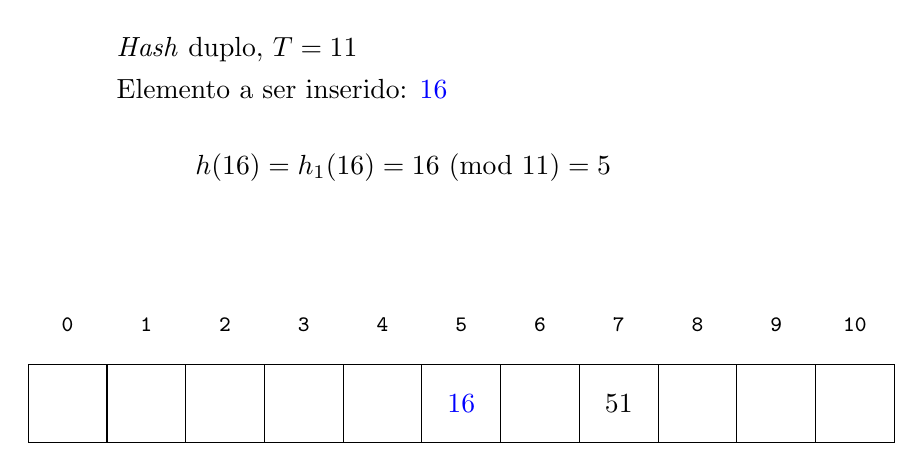
\begin{tikzpicture}
            \draw (0, 1) grid (11, 2);

            \node at (0.5, 2.5) { \tt \footnotesize 0 };
            \node at (1.5, 2.5) { \tt \footnotesize 1 };
            \node at (2.5, 2.5) { \tt \footnotesize 2 };
            \node at (3.5, 2.5) { \tt \footnotesize 3 };
            \node at (4.5, 2.5) { \tt \footnotesize 4 };
            \node at (5.5, 2.5) { \tt \footnotesize 5 };
            \node at (6.5, 2.5) { \tt \footnotesize 6 };
            \node at (7.5, 2.5) { \tt \footnotesize 7 };
            \node at (8.5, 2.5) { \tt \footnotesize 8 };
            \node at (9.5, 2.5) { \tt \footnotesize 9 };
            \node at (10.5, 2.5) { \tt \footnotesize 10 };

            \node[anchor=west] at (1, 6) { \textit{Hash} duplo, $T = 11$ };
            \node[anchor=west] at (1, 5.5) { Elemento a ser inserido: \textcolor{blue}{$16$} };

            \node[anchor=west] at (2, 4.5) { $h(16) = h_1(16) = 16\ (\mbox{mod}\ 11) = 5$ };

            \node at (5.5, 1.5) { \textcolor{blue}{$16$} };
            \node at (7.5, 1.5) { \textcolor{black}{$51$} };
        \end{tikzpicture}
    \end{figure}

\end{frame}

\begin{frame}{Exemplo de inserção utilizando \textit{hash} duplo} 

    \begin{figure}
        \begin{tikzpicture}
            \draw (0, 1) grid (11, 2);

            \node at (0.5, 2.5) { \tt \footnotesize 0 };
            \node at (1.5, 2.5) { \tt \footnotesize 1 };
            \node at (2.5, 2.5) { \tt \footnotesize 2 };
            \node at (3.5, 2.5) { \tt \footnotesize 3 };
            \node at (4.5, 2.5) { \tt \footnotesize 4 };
            \node at (5.5, 2.5) { \tt \footnotesize 5 };
            \node at (6.5, 2.5) { \tt \footnotesize 6 };
            \node at (7.5, 2.5) { \tt \footnotesize 7 };
            \node at (8.5, 2.5) { \tt \footnotesize 8 };
            \node at (9.5, 2.5) { \tt \footnotesize 9 };
            \node at (10.5, 2.5) { \tt \footnotesize 10 };

            \node[anchor=west] at (1, 6) { \textit{Hash} duplo, $T = 11$ };
            \node[anchor=west] at (1, 5.5) { Elemento a ser inserido: \textcolor{blue}{$76$} };

%            \node[anchor=west] at (2, 4.5) { $h(16) = 16\ (\mbox{mod}\ 11) = 5$ };

            \node at (5.5, 1.5) { \textcolor{black}{$16$} };
            \node at (7.5, 1.5) { \textcolor{black}{$51$} };
        \end{tikzpicture}
    \end{figure}

\end{frame}

\begin{frame}{Exemplo de inserção utilizando \textit{hash} duplo} 

    \begin{figure}
        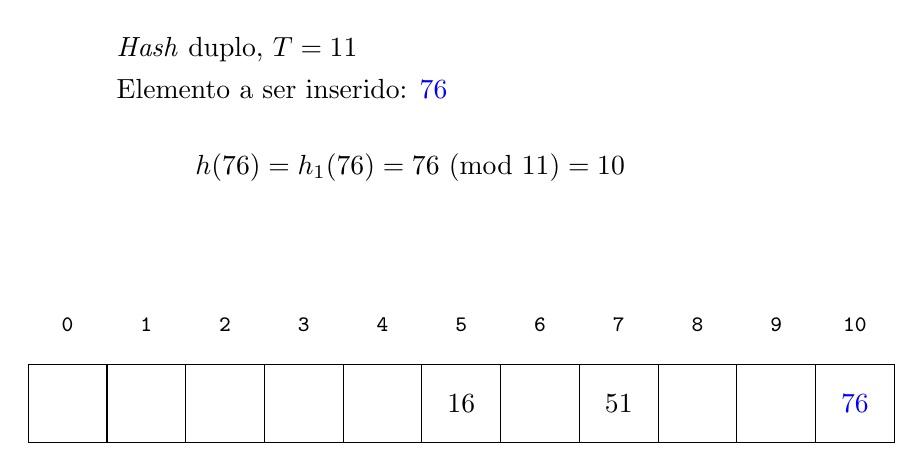
\begin{tikzpicture}
            \draw (0, 1) grid (11, 2);

            \node at (0.5, 2.5) { \tt \footnotesize 0 };
            \node at (1.5, 2.5) { \tt \footnotesize 1 };
            \node at (2.5, 2.5) { \tt \footnotesize 2 };
            \node at (3.5, 2.5) { \tt \footnotesize 3 };
            \node at (4.5, 2.5) { \tt \footnotesize 4 };
            \node at (5.5, 2.5) { \tt \footnotesize 5 };
            \node at (6.5, 2.5) { \tt \footnotesize 6 };
            \node at (7.5, 2.5) { \tt \footnotesize 7 };
            \node at (8.5, 2.5) { \tt \footnotesize 8 };
            \node at (9.5, 2.5) { \tt \footnotesize 9 };
            \node at (10.5, 2.5) { \tt \footnotesize 10 };

            \node[anchor=west] at (1, 6) { \textit{Hash} duplo, $T = 11$ };
            \node[anchor=west] at (1, 5.5) { Elemento a ser inserido: \textcolor{blue}{$76$} };

            \node[anchor=west] at (2, 4.5) { $h(76) = h_1(76) = 76\ (\mbox{mod}\ 11) = 10$ };

            \node at (5.5, 1.5) { \textcolor{black}{$16$} };
            \node at (7.5, 1.5) { \textcolor{black}{$51$} };
            \node at (10.5, 1.5) { \textcolor{blue}{$76$} };
        \end{tikzpicture}
    \end{figure}

\end{frame}

\begin{frame}{Exemplo de inserção utilizando \textit{hash} duplo} 

    \begin{figure}
        \begin{tikzpicture}
            \draw (0, 1) grid (11, 2);

            \node at (0.5, 2.5) { \tt \footnotesize 0 };
            \node at (1.5, 2.5) { \tt \footnotesize 1 };
            \node at (2.5, 2.5) { \tt \footnotesize 2 };
            \node at (3.5, 2.5) { \tt \footnotesize 3 };
            \node at (4.5, 2.5) { \tt \footnotesize 4 };
            \node at (5.5, 2.5) { \tt \footnotesize 5 };
            \node at (6.5, 2.5) { \tt \footnotesize 6 };
            \node at (7.5, 2.5) { \tt \footnotesize 7 };
            \node at (8.5, 2.5) { \tt \footnotesize 8 };
            \node at (9.5, 2.5) { \tt \footnotesize 9 };
            \node at (10.5, 2.5) { \tt \footnotesize 10 };

            \node[anchor=west] at (1, 6) { \textit{Hash} duplo, $T = 11$ };
            \node[anchor=west] at (1, 5.5) { Elemento a ser inserido: \textcolor{blue}{$35$} };

%            \node[anchor=west] at (2, 4.5) { $h(76) = 76\ (\mbox{mod}\ 11) = 10$ };

            \node at (5.5, 1.5) { \textcolor{black}{$16$} };
            \node at (7.5, 1.5) { \textcolor{black}{$51$} };
            \node at (10.5, 1.5) { \textcolor{black}{$76$} };
        \end{tikzpicture}
    \end{figure}

\end{frame}

\begin{frame}{Exemplo de inserção utilizando \textit{hash} duplo} 

    \begin{figure}
        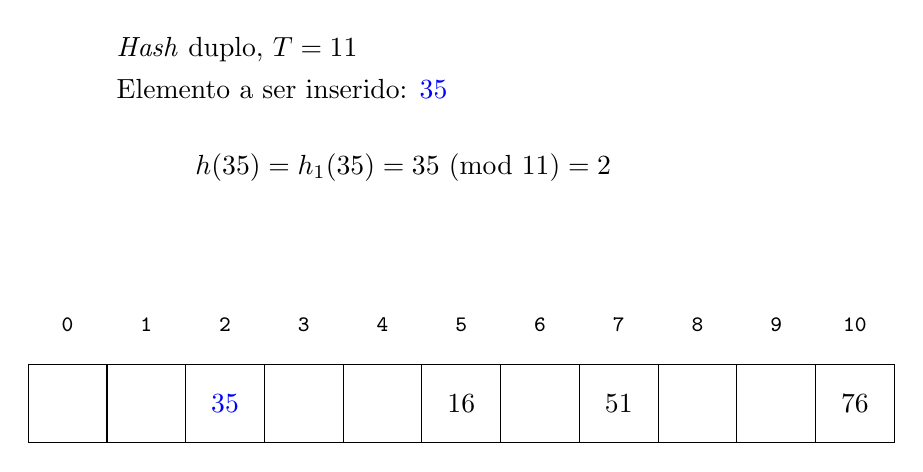
\begin{tikzpicture}
            \draw (0, 1) grid (11, 2);

            \node at (0.5, 2.5) { \tt \footnotesize 0 };
            \node at (1.5, 2.5) { \tt \footnotesize 1 };
            \node at (2.5, 2.5) { \tt \footnotesize 2 };
            \node at (3.5, 2.5) { \tt \footnotesize 3 };
            \node at (4.5, 2.5) { \tt \footnotesize 4 };
            \node at (5.5, 2.5) { \tt \footnotesize 5 };
            \node at (6.5, 2.5) { \tt \footnotesize 6 };
            \node at (7.5, 2.5) { \tt \footnotesize 7 };
            \node at (8.5, 2.5) { \tt \footnotesize 8 };
            \node at (9.5, 2.5) { \tt \footnotesize 9 };
            \node at (10.5, 2.5) { \tt \footnotesize 10 };

            \node[anchor=west] at (1, 6) { \textit{Hash} duplo, $T = 11$ };
            \node[anchor=west] at (1, 5.5) { Elemento a ser inserido: \textcolor{blue}{$35$} };

            \node[anchor=west] at (2, 4.5) { $h(35) = h_1(35) = 35\ (\mbox{mod}\ 11) = 2$ };

            \node at (2.5, 1.5) { \textcolor{blue}{$35$} };
            \node at (5.5, 1.5) { \textcolor{black}{$16$} };
            \node at (7.5, 1.5) { \textcolor{black}{$51$} };
            \node at (10.5, 1.5) { \textcolor{black}{$76$} };
        \end{tikzpicture}
    \end{figure}

\end{frame}

\begin{frame}{Exemplo de inserção utilizando \textit{hash} duplo} 

    \begin{figure}
        \begin{tikzpicture}
            \draw (0, 1) grid (11, 2);

            \node at (0.5, 2.5) { \tt \footnotesize 0 };
            \node at (1.5, 2.5) { \tt \footnotesize 1 };
            \node at (2.5, 2.5) { \tt \footnotesize 2 };
            \node at (3.5, 2.5) { \tt \footnotesize 3 };
            \node at (4.5, 2.5) { \tt \footnotesize 4 };
            \node at (5.5, 2.5) { \tt \footnotesize 5 };
            \node at (6.5, 2.5) { \tt \footnotesize 6 };
            \node at (7.5, 2.5) { \tt \footnotesize 7 };
            \node at (8.5, 2.5) { \tt \footnotesize 8 };
            \node at (9.5, 2.5) { \tt \footnotesize 9 };
            \node at (10.5, 2.5) { \tt \footnotesize 10 };

            \node[anchor=west] at (1, 6) { \textit{Hash} duplo, $T = 11$ };
            \node[anchor=west] at (1, 5.5) { Elemento a ser inserido: \textcolor{blue}{$-6$} };

%            \node[anchor=west] at (2, 4.5) { $h(35) = 35\ (\mbox{mod}\ 11) = 2$ };

            \node at (2.5, 1.5) { \textcolor{black}{$35$} };
            \node at (5.5, 1.5) { \textcolor{black}{$16$} };
            \node at (7.5, 1.5) { \textcolor{black}{$51$} };
            \node at (10.5, 1.5) { \textcolor{black}{$76$} };
        \end{tikzpicture}
    \end{figure}

\end{frame}

\begin{frame}{Exemplo de inserção utilizando \textit{hash} duplo} 

    \begin{figure}
        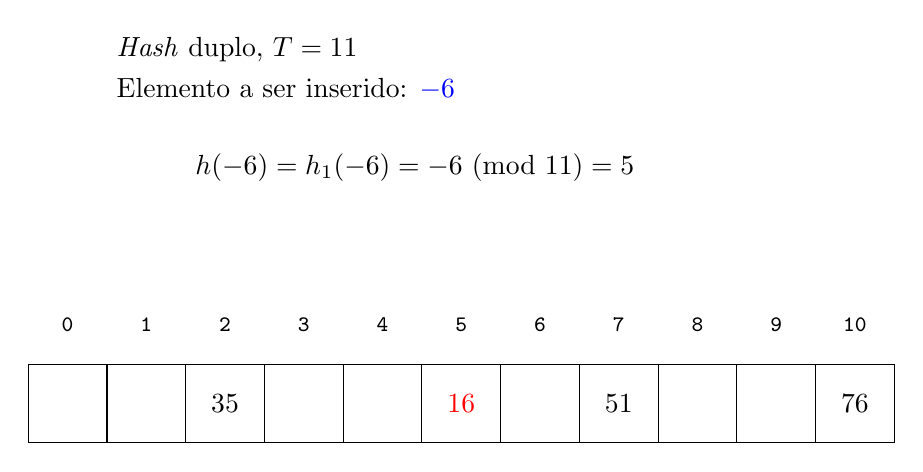
\begin{tikzpicture}
            \draw (0, 1) grid (11, 2);

            \node at (0.5, 2.5) { \tt \footnotesize 0 };
            \node at (1.5, 2.5) { \tt \footnotesize 1 };
            \node at (2.5, 2.5) { \tt \footnotesize 2 };
            \node at (3.5, 2.5) { \tt \footnotesize 3 };
            \node at (4.5, 2.5) { \tt \footnotesize 4 };
            \node at (5.5, 2.5) { \tt \footnotesize 5 };
            \node at (6.5, 2.5) { \tt \footnotesize 6 };
            \node at (7.5, 2.5) { \tt \footnotesize 7 };
            \node at (8.5, 2.5) { \tt \footnotesize 8 };
            \node at (9.5, 2.5) { \tt \footnotesize 9 };
            \node at (10.5, 2.5) { \tt \footnotesize 10 };

            \node[anchor=west] at (1, 6) { \textit{Hash} duplo, $T = 11$ };
            \node[anchor=west] at (1, 5.5) { Elemento a ser inserido: \textcolor{blue}{$-6$} };

            \node[anchor=west] at (2, 4.5) { $h(-6) = h_1(-6) = -6\ (\mbox{mod}\ 11) = 5$ };

            \node at (2.5, 1.5) { \textcolor{black}{$35$} };
            \node at (5.5, 1.5) { \textcolor{red}{$16$} };
            \node at (7.5, 1.5) { \textcolor{black}{$51$} };
            \node at (10.5, 1.5) { \textcolor{black}{$76$} };
        \end{tikzpicture}
    \end{figure}

\end{frame}

\begin{frame}{Exemplo de inserção utilizando \textit{hash} duplo} 

    \begin{figure}
        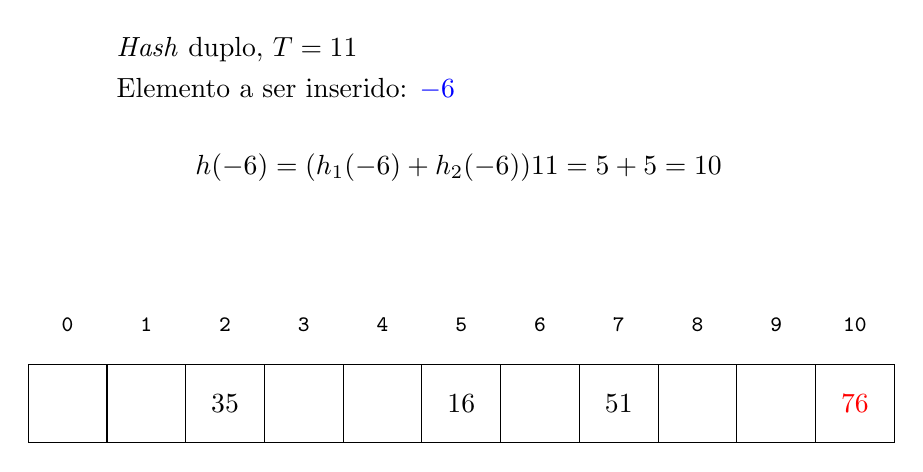
\begin{tikzpicture}
            \draw (0, 1) grid (11, 2);

            \node at (0.5, 2.5) { \tt \footnotesize 0 };
            \node at (1.5, 2.5) { \tt \footnotesize 1 };
            \node at (2.5, 2.5) { \tt \footnotesize 2 };
            \node at (3.5, 2.5) { \tt \footnotesize 3 };
            \node at (4.5, 2.5) { \tt \footnotesize 4 };
            \node at (5.5, 2.5) { \tt \footnotesize 5 };
            \node at (6.5, 2.5) { \tt \footnotesize 6 };
            \node at (7.5, 2.5) { \tt \footnotesize 7 };
            \node at (8.5, 2.5) { \tt \footnotesize 8 };
            \node at (9.5, 2.5) { \tt \footnotesize 9 };
            \node at (10.5, 2.5) { \tt \footnotesize 10 };

            \node[anchor=west] at (1, 6) { \textit{Hash} duplo, $T = 11$ };
            \node[anchor=west] at (1, 5.5) { Elemento a ser inserido: \textcolor{blue}{$-6$} };

            \node[anchor=west] at (2, 4.5) { $h(-6) = \Mod{(h_1(-6) + h_2(-6))}{11} = 5 + 5 = 10$ };

            \node at (2.5, 1.5) { \textcolor{black}{$35$} };
            \node at (5.5, 1.5) { \textcolor{black}{$16$} };
            \node at (7.5, 1.5) { \textcolor{black}{$51$} };
            \node at (10.5, 1.5) { \textcolor{red}{$76$} };
        \end{tikzpicture}
    \end{figure}

\end{frame}

\begin{frame}{Exemplo de inserção utilizando \textit{hash} duplo} 

    \begin{figure}
        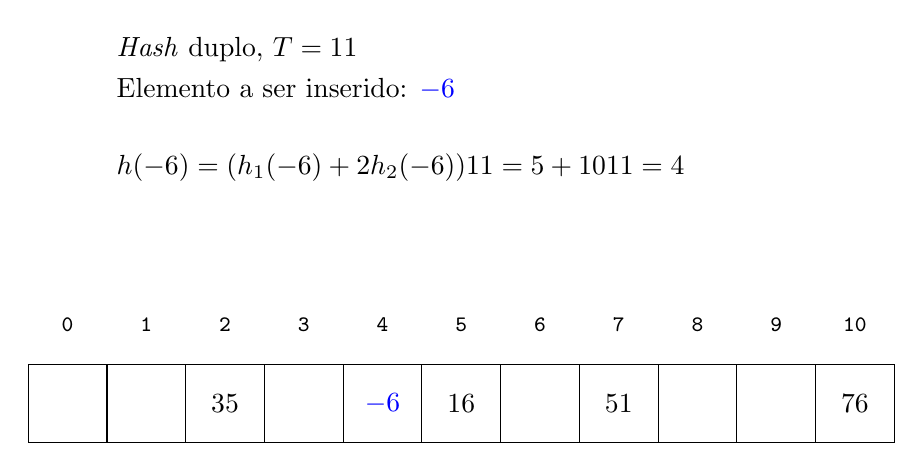
\begin{tikzpicture}
            \draw (0, 1) grid (11, 2);

            \node at (0.5, 2.5) { \tt \footnotesize 0 };
            \node at (1.5, 2.5) { \tt \footnotesize 1 };
            \node at (2.5, 2.5) { \tt \footnotesize 2 };
            \node at (3.5, 2.5) { \tt \footnotesize 3 };
            \node at (4.5, 2.5) { \tt \footnotesize 4 };
            \node at (5.5, 2.5) { \tt \footnotesize 5 };
            \node at (6.5, 2.5) { \tt \footnotesize 6 };
            \node at (7.5, 2.5) { \tt \footnotesize 7 };
            \node at (8.5, 2.5) { \tt \footnotesize 8 };
            \node at (9.5, 2.5) { \tt \footnotesize 9 };
            \node at (10.5, 2.5) { \tt \footnotesize 10 };

            \node[anchor=west] at (1, 6) { \textit{Hash} duplo, $T = 11$ };
            \node[anchor=west] at (1, 5.5) { Elemento a ser inserido: \textcolor{blue}{$-6$} };

            \node[anchor=west] at (1, 4.5) { $h(-6) = \Mod{(h_1(-6) + 2h_2(-6))}{11} = \Mod{5 + 10}{11} = 4$ };

            \node at (2.5, 1.5) { \textcolor{black}{$35$} };
            \node at (4.5, 1.5) { \textcolor{blue}{$-6$} };
            \node at (5.5, 1.5) { \textcolor{black}{$16$} };
            \node at (7.5, 1.5) { \textcolor{black}{$51$} };
            \node at (10.5, 1.5) { \textcolor{black}{$76$} };
        \end{tikzpicture}
    \end{figure}

\end{frame}


\begin{frame}{Exemplo de inserção utilizando \textit{hash} duplo} 

    \begin{figure}
        \begin{tikzpicture}
            \draw (0, 1) grid (11, 2);

            \node at (0.5, 2.5) { \tt \footnotesize 0 };
            \node at (1.5, 2.5) { \tt \footnotesize 1 };
            \node at (2.5, 2.5) { \tt \footnotesize 2 };
            \node at (3.5, 2.5) { \tt \footnotesize 3 };
            \node at (4.5, 2.5) { \tt \footnotesize 4 };
            \node at (5.5, 2.5) { \tt \footnotesize 5 };
            \node at (6.5, 2.5) { \tt \footnotesize 6 };
            \node at (7.5, 2.5) { \tt \footnotesize 7 };
            \node at (8.5, 2.5) { \tt \footnotesize 8 };
            \node at (9.5, 2.5) { \tt \footnotesize 9 };
            \node at (10.5, 2.5) { \tt \footnotesize 10 };

            \node[anchor=west] at (1, 6) { \textit{Hash} duplo, $T = 11$ };
            \node[anchor=west] at (1, 5.5) { Elemento a ser inserido: \textcolor{blue}{$49$} };

            \node at (2.5, 1.5) { \textcolor{black}{$35$} };
            \node at (4.5, 1.5) { \textcolor{black}{$-6$} };
            \node at (5.5, 1.5) { \textcolor{black}{$16$} };
            \node at (7.5, 1.5) { \textcolor{black}{$51$} };
            \node at (10.5, 1.5) { \textcolor{black}{$76$} };
        \end{tikzpicture}
    \end{figure}

\end{frame}

\begin{frame}{Exemplo de inserção utilizando \textit{hash} duplo} 

    \begin{figure}
        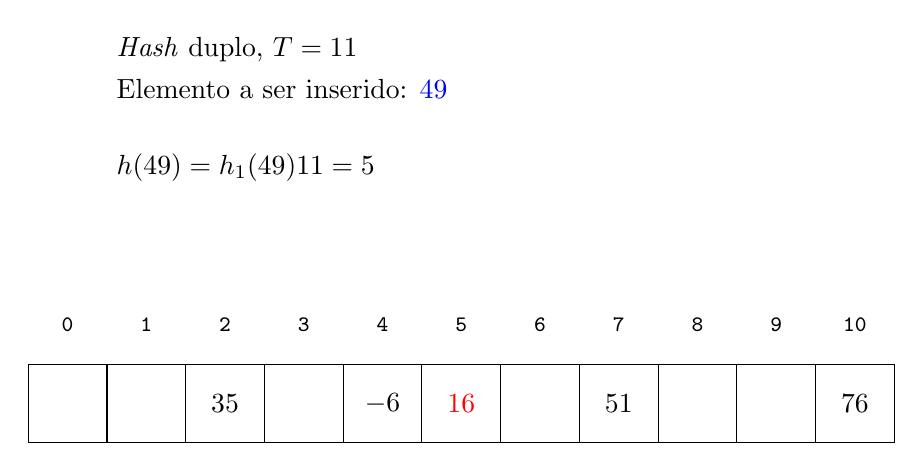
\begin{tikzpicture}
            \draw (0, 1) grid (11, 2);

            \node at (0.5, 2.5) { \tt \footnotesize 0 };
            \node at (1.5, 2.5) { \tt \footnotesize 1 };
            \node at (2.5, 2.5) { \tt \footnotesize 2 };
            \node at (3.5, 2.5) { \tt \footnotesize 3 };
            \node at (4.5, 2.5) { \tt \footnotesize 4 };
            \node at (5.5, 2.5) { \tt \footnotesize 5 };
            \node at (6.5, 2.5) { \tt \footnotesize 6 };
            \node at (7.5, 2.5) { \tt \footnotesize 7 };
            \node at (8.5, 2.5) { \tt \footnotesize 8 };
            \node at (9.5, 2.5) { \tt \footnotesize 9 };
            \node at (10.5, 2.5) { \tt \footnotesize 10 };

            \node[anchor=west] at (1, 6) { \textit{Hash} duplo, $T = 11$ };
            \node[anchor=west] at (1, 5.5) { Elemento a ser inserido: \textcolor{blue}{$49$} };

            \node[anchor=west] at (1, 4.5) { $h(49) = \Mod{h_1(49)}{11} = 5$ };

            \node at (2.5, 1.5) { \textcolor{black}{$35$} };
            \node at (4.5, 1.5) { \textcolor{black}{$-6$} };
            \node at (5.5, 1.5) { \textcolor{red}{$16$} };
            \node at (7.5, 1.5) { \textcolor{black}{$51$} };
            \node at (10.5, 1.5) { \textcolor{black}{$76$} };
        \end{tikzpicture}
    \end{figure}

\end{frame}



\begin{frame}{Exemplo de inserção utilizando \textit{hash} duplo} 

    \begin{figure}
        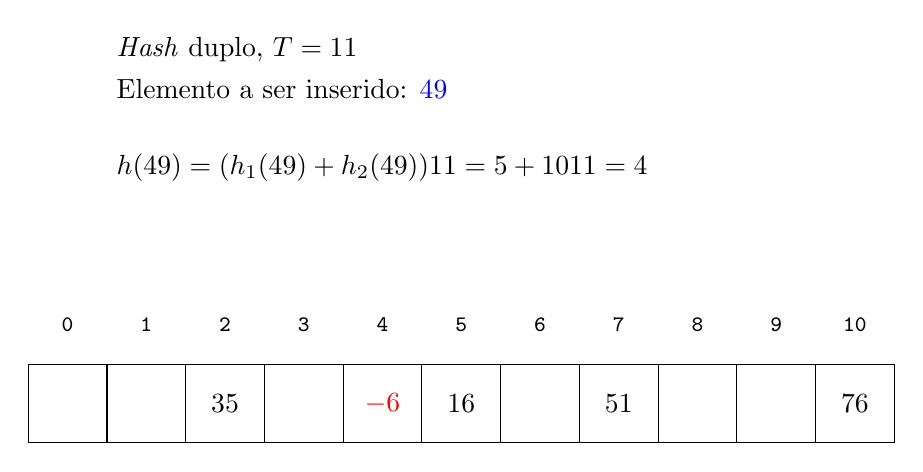
\begin{tikzpicture}
            \draw (0, 1) grid (11, 2);

            \node at (0.5, 2.5) { \tt \footnotesize 0 };
            \node at (1.5, 2.5) { \tt \footnotesize 1 };
            \node at (2.5, 2.5) { \tt \footnotesize 2 };
            \node at (3.5, 2.5) { \tt \footnotesize 3 };
            \node at (4.5, 2.5) { \tt \footnotesize 4 };
            \node at (5.5, 2.5) { \tt \footnotesize 5 };
            \node at (6.5, 2.5) { \tt \footnotesize 6 };
            \node at (7.5, 2.5) { \tt \footnotesize 7 };
            \node at (8.5, 2.5) { \tt \footnotesize 8 };
            \node at (9.5, 2.5) { \tt \footnotesize 9 };
            \node at (10.5, 2.5) { \tt \footnotesize 10 };

            \node[anchor=west] at (1, 6) { \textit{Hash} duplo, $T = 11$ };
            \node[anchor=west] at (1, 5.5) { Elemento a ser inserido: \textcolor{blue}{$49$} };

            \node[anchor=west] at (1, 4.5) { $h(49) = \Mod{(h_1(49) + h_2(49))}{11} = \Mod{5 + 10}{11} = 4 $ };

            \node at (2.5, 1.5) { \textcolor{black}{$35$} };
            \node at (4.5, 1.5) { \textcolor{red}{$-6$} };
            \node at (5.5, 1.5) { \textcolor{black}{$16$} };
            \node at (7.5, 1.5) { \textcolor{black}{$51$} };
            \node at (10.5, 1.5) { \textcolor{black}{$76$} };
        \end{tikzpicture}
    \end{figure}

\end{frame}

\begin{frame}{Exemplo de inserção utilizando \textit{hash} duplo} 

    \begin{figure}
        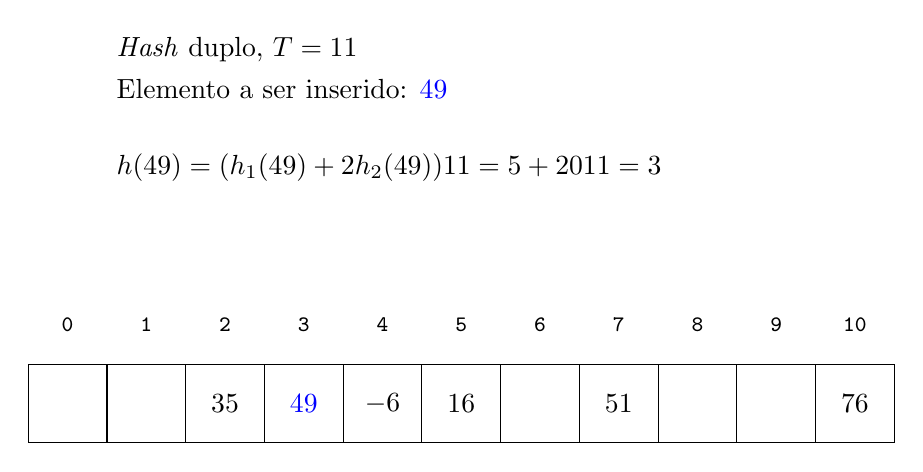
\begin{tikzpicture}
            \draw (0, 1) grid (11, 2);

            \node at (0.5, 2.5) { \tt \footnotesize 0 };
            \node at (1.5, 2.5) { \tt \footnotesize 1 };
            \node at (2.5, 2.5) { \tt \footnotesize 2 };
            \node at (3.5, 2.5) { \tt \footnotesize 3 };
            \node at (4.5, 2.5) { \tt \footnotesize 4 };
            \node at (5.5, 2.5) { \tt \footnotesize 5 };
            \node at (6.5, 2.5) { \tt \footnotesize 6 };
            \node at (7.5, 2.5) { \tt \footnotesize 7 };
            \node at (8.5, 2.5) { \tt \footnotesize 8 };
            \node at (9.5, 2.5) { \tt \footnotesize 9 };
            \node at (10.5, 2.5) { \tt \footnotesize 10 };

            \node[anchor=west] at (1, 6) { \textit{Hash} duplo, $T = 11$ };
            \node[anchor=west] at (1, 5.5) { Elemento a ser inserido: \textcolor{blue}{$49$} };

            \node[anchor=west] at (1, 4.5) { $h(49) = \Mod{(h_1(49) + 2h_2(49))}{11} = \Mod{5 + 20}{11} = 3 $ };

            \node at (2.5, 1.5) { \textcolor{black}{$35$} };
            \node at (3.5, 1.5) { \textcolor{blue}{$49$} };
            \node at (4.5, 1.5) { \textcolor{black}{$-6$} };
            \node at (5.5, 1.5) { \textcolor{black}{$16$} };
            \node at (7.5, 1.5) { \textcolor{black}{$51$} };
            \node at (10.5, 1.5) { \textcolor{black}{$76$} };
        \end{tikzpicture}
    \end{figure}

\end{frame}
